%=================================================================
% Joint Service Chain Deployment and Manager Placement in NFV
% MDPI (Future Internet) LaTeX manuscript.
% Uses the MDPI class in Definitions/ (download the latest from
% https://www.mdpi.com/authors/latex before final submission).
%=================================================================
\documentclass[futureinternet,article,submit,pdftex,moreauthors]{Definitions/mdpi}

% Extra packages (most are already loaded by the MDPI class: amsmath, float,
% booktabs, graphicx, multirow, xcolor, hyperref).
\usepackage{amssymb}
\usepackage{tabularx}
\usepackage{algorithm}
\usepackage{algpseudocode}

\firstpage{1}
\makeatletter
\setcounter{page}{\@firstpage}
\makeatother
\pubvolume{1}
\issuenum{1}
\articlenumber{0}
\pubyear{2026}
\copyrightyear{2026}
\history{Received: ; Accepted: ; Published: }

%=================================================================
\Title{Joint Service Chain Deployment and Manager Placement in NFV}

\Author{Parham Alvani $^{1}$ and Bahador Bakhshi $^{1,}$*}

\AuthorNames{Parham Alvani and Bahador Bakhshi}

\address{%
$^{1}$ \quad Amirkabir University of Technology, Tehran, Iran;
parham.alvani@aut.ac.ir (P.A.); bbakhshi@aut.ac.ir (B.B.)}

\corres{Correspondence: bbakhshi@aut.ac.ir}

\abstract{Network operators deploying service function chains (SFCs) with Network
Function Virtualization (NFV) must also provide each chain with a VNF Manager
(VNFM) under capacity, latency-radius, and co-location constraints. Most prior
work optimizes VNF placement first and assigns managers afterward. We show that
this \emph{disjoint} approach is not merely suboptimal but frequently
\emph{infeasible}: management-blind VNF layouts strand whole chains because no
admissible manager exists for the chosen placement. We formulate the joint SFC
deployment and VNFM placement problem (JSD-MP) as an Integer Linear Program,
show it is NP-hard, and propose MASMAN, a polynomial-time heuristic that makes
VNF placement management-aware (a Viterbi-style dynamic program) and then
consolidates managers with Tabu search. Against an exact CPLEX solver---which
already exhausts memory at around a dozen chains---the heuristic stays within
roughly 18\% of the optimal revenue while scaling to hundreds of chains. Finally,
we characterize
\emph{when} joint placement matters: its benefit is a feasibility effect that
appears precisely when management constraints bind, and is negligible under
slack management or when raw compute saturates the network.}

\keyword{network function virtualization; service function chaining; VNF
placement; VNF manager placement; joint optimization; integer linear
programming; heuristic; feasibility}

\begin{document}

\section{Introduction}\label{sec:introduction}
\input{introduction}

\section{Related Work}\label{sec:related-works}
\input{related-works}

\section{System Model and Problem Statement}\label{sec:system-model}
\input{system}

\section{Problem Formulation}\label{sec:formulation}
In this section, the JSD-MP problem is formulated as a MILP model. First the
variables of the model are introduced, then the constraints are discussed, and
finally the objective is presented.

The variables are listed in Table~\ref{tbl:variables}. \(x_r\) is a binary
variable for the acceptance of demand \(r \in R\). The integer variable
\(y_{it}\) is the number of VNFs of type \(t \in T\) on server \(i\). The binary
variable \(z^t_{vi}\) indicates whether an instance of VNF type \(t\) serves node
\(v\) on server \(i\). The integer variable \(\bar{y}_i\) is the number of VNFMs
placed on server \(i\), and the binary variable \(\bar{z}_{ri}\) represents the
VNFM assignment of a chain. Finally, \(\pi^{(u,v)}_{ij}\) and \(\bar{\pi}^v_{ij}\)
are binary variables indicating that virtual link \((u,v)\) is mapped on physical
link \((i,j)\) and that link \((i,j)\) is used to manage VNF \(v\), respectively.

\begin{table}[H]
\caption{Variables.}
\label{tbl:variables}
\small
\begin{tabularx}{\textwidth}{cX}
\toprule
\textbf{Variable} & \textbf{Description} \\
\midrule
\(x_r\) & 1 if the SFC request \(r\) is accepted; otherwise 0 \\
\(y_{it}\) & number of VNF instances of type \(t \in T\) set up on server \(i \in V^p\) \\
\(z^t_{vi}\) & 1 if VNF node \(v \in \bigcup_{r=1}^{R} V^s_r\) is served by a VNF instance of type \(t \in T\) on server \(i \in V^p\) \\
\(\bar{y}_i\) & number of VNFMs set up on server \(i \in V^p\) (each with its capacity and license fee) \\
\(\bar{z}_{ri}\) & 1 if SFC \(r\) is assigned to a VNFM on server \(i \in V^p\) \\
\(\pi^{(u,v)}_{ij}\) & 1 if virtual link \((u,v)\) is routed on physical link \((i,j)\) \\
\(\bar{\pi}^v_{ij}\) & 1 if the management of VNF node \(v\) is routed on physical link \((i,j)\) \\
\bottomrule
\end{tabularx}
\end{table}

Each node has limited installed memory; each VNF instance (by its type) and each
VNFM uses a specific amount. Equation~\eqref{eq:node-memory} limits the used
memory of each node by its installed memory.

\begin{equation}\label{eq:node-memory}
\sum_{t \in T} y_{it}\, m^s_t + \bar{y}_i\, m^m \le m^p_i \quad \forall i \in V^p
\end{equation}

Each node has limited processing power in CPU cores.
Equation~\eqref{eq:node-cpu} limits the used processing power of each node by its
installed CPUs.

\begin{equation}\label{eq:node-cpu}
\sum_{t \in T} y_{it}\, c^s_t + \bar{y}_i\, c^m \le c^p_i \quad \forall i \in V^p
\end{equation}

If a chain's node is served on a physical node, a VNF instance must be set up on
it. Equation~\eqref{eq:service-place} controls this relationship.

\begin{equation}\label{eq:service-place}
\sum_{v \in \bigcup_{r=1}^{R} V^s_r} z^t_{vi} \le y_{it}
\quad \forall i \in V^p,\ \forall t \in T
\end{equation}

Equations~\eqref{eq:service} and \eqref{eq:manager} accept a chain only if all of
its nodes are placed on physical servers and it has an assigned VNFM.

\begin{equation}\label{eq:service}
x_r = \sum_{t \in T} \sum_{i \in V^p} z^t_{vi}
\quad \forall v \in V^s_r,\ \forall r \in R
\end{equation}

\begin{equation}\label{eq:manager}
x_r = \sum_{i \in V^p} \bar{z}_{ri} \quad \forall r \in R
\end{equation}

Equation~\eqref{eq:manager-capacity} limits manager capacity.

\begin{equation}\label{eq:manager-capacity}
\sum_{r \in R} \bar{z}_{ri} \cdot |V^s_r| \le \kappa \cdot \bar{y}_i
\quad \forall i \in V^p
\end{equation}

Equation~\eqref{eq:type} assures each chain's node is served by a VNF of its type.

\begin{equation}\label{eq:type}
z^t_{vi} \le \tau(v, t)
\quad \forall i \in V^p,\ \forall t \in T,\ \forall v \in \bigcup_{r \in R} V^s_r
\end{equation}

Each physical server has a set of servers that cannot manage it.
Equation~\eqref{eq:mgmt-relationship} represents this.

\begin{equation}\label{eq:mgmt-relationship}
\begin{aligned}
& 1 - z^t_{vi} + \bar{z}_{rj} = 0, \\
& \forall i, j \in V^p \text{ with } \eta_{i,j} = 1,\ \forall r \in R,\ \forall v \in V^s_r,\ \forall t \in T
\end{aligned}
\end{equation}

Equations~\eqref{eq:flow} and \eqref{eq:mgmt-flow} express flow conservation on
service and management links, respectively.

\begin{equation}\label{eq:flow}
\begin{aligned}
& \sum_{(i,j) \in E^p} \pi^{(u,v)}_{ij} - \sum_{(j,i) \in E^p} \pi^{(u,v)}_{ji} = \sum_{t \in T} z^t_{ui} - \sum_{t \in T} z^t_{vi}, \\
& \forall i \in V^p,\ (u,v) \in E^s_r,\ r \in R
\end{aligned}
\end{equation}

\begin{equation}\label{eq:mgmt-flow}
\begin{aligned}
& \sum_{(i,j) \in E^p} \bar{\pi}^v_{ij} - \sum_{(j,i) \in E^p} \bar{\pi}^v_{ji} = \sum_{t \in T} z^t_{vi} - \bar{z}_{ri}, \\
& \forall i \in V^p,\ v \in V^s_r,\ r \in R
\end{aligned}
\end{equation}

Equation~\eqref{eq:link-bw} limits the consumed bandwidth of each link by its
capacity.

\begin{equation}\label{eq:link-bw}
\begin{aligned}
& \sum_{v \in \bigcup_{r \in R} V^s_r} \bar{\pi}^v_{ij} \cdot b^m + \sum_{r \in R} \sum_{(u,v) \in E^s_r} \pi^{(u,v)}_{ij} \cdot b^s_{(u,v),r} \le b^p_{ij}, \\
& \forall (i,j) \in E^p
\end{aligned}
\end{equation}

Equation~\eqref{eq:radius} controls the management radius.

\begin{equation}\label{eq:radius}
\sum_{(i,j) \in E^p} \bar{\pi}^v_{ij} \le \rho
\quad \forall v \in \bigcup_{r \in R} V^s_r
\end{equation}

The objective is to maximize the profit from placing chains:

\begin{equation}\label{eq:objective}
\max \sum_{r \in R} c_r\, x_r - \sum_{i \in V^p} \phi \cdot \bar{y}_i
\end{equation}

The problem is an ILP and can be reduced to bin packing, so it is NP-hard.


\section{Proposed Solution}\label{sec:solution}
The JSD-MP problem is NP-hard, so solving the ILP of
Section~\ref{sec:formulation} to optimality is intractable at the scale of a real
data center. In this section we propose MASMAN, a polynomial-time heuristic that
produces a near-optimal placement quickly enough to be used for admission control
on large infrastructures with many nodes and requests.

\subsection{Maximizing the Accepted SFC Requests with Management Constraints (MASMAN)}
Placing a chain involves two coupled sub-problems: \emph{VNF placement} (locating
the chain's VNFs) and \emph{VNFM placement} (locating the chain's manager). MASMAN
solves them in two phases, but keeps the first phase management-aware so that the
second phase rarely fails: before placement we reserve at least one VNFM's worth of
resources on every physical node, so a layout chosen in phase one cannot strand the
chain for lack of room to host its manager.

The first phase places the VNFs with the dynamic-programming algorithm of
Bari~\textit{et~al.}~\cite{Bari2015}. For each chain this algorithm finds a
minimum-cost placement by building a multi-stage graph---one stage per VNF of the
chain, with the candidate physical nodes as the vertices of each stage---and
running a Viterbi-style shortest-path recursion over it: the optimal placement up
to stage \(i\) at node \(n\) is obtained from the best placement at stage
\(i-1\), since a minimum-cost path is composed of minimum-cost sub-paths. The
original algorithm is management-blind; we make it management-aware by admitting a
candidate node at a stage only when, in addition to the VNF's compute and
bandwidth requirements, the reserved manager resources and the co-location
(\(\eta\)) and radius (\(\rho\)) constraints can still be satisfied for the
partial layout.

The second phase assigns each chain an admissible VNFM and then applies a Tabu
search to \emph{consolidate} managers and cut the license cost: it repeatedly
tries to merge the chains of one VNFM node onto another, accepting a merge when it
remains feasible and lowers the total license cost, while a tabu list prevents
re-examining recently tried node pairs. The two phases are detailed in
Algorithm~\ref{alg:masman}.

\begin{algorithm}
  \caption{MASMAN --- management-aware VNF placement (phase 1)}
  \label{alg:masman}
  \begin{algorithmic}[1]
    \Require{$chains$, $topology$}
    \Function{masman\_placement}{$chains, topology$}
    \ForAll{$chain \in chains$}
      \State{$L \gets len(chain)$}\Comment{number of VNFs in the chain}
      \State{$cost[\cdot,\cdot] \gets +\infty$;\quad $prev[\cdot,\cdot] \gets \textsc{nil}$}
      \ForAll{$n \in topology.nodes$}\Comment{stage 0: first VNF, no predecessor}
        \If{$hasEnoughResource(n, chain[0])$}
          \State{$cost[0, n] \gets nodeCost(n, chain[0])$}
        \EndIf
      \EndFor
      \For{$i \gets 1, L - 1$}\Comment{remaining stages}
        \ForAll{$n \in topology.nodes$}
          \ForAll{$k \in topology.nodes$}
            \If{$cost[i-1, k] < \infty$ \textbf{and} $feasible(i{-}1, k \rightarrow i, n)$}
              \State{$c \gets cost[i-1, k] + linkCost(k, n) + nodeCost(n, chain[i])$}
              \If{$c < cost[i, n]$}\Comment{keep the minimum-cost sub-path}
                \State{$cost[i, n] \gets c$;\quad $prev[i, n] \gets k$}
              \EndIf
            \EndIf
          \EndFor
        \EndFor
      \EndFor
      \State{$n^\star \gets \arg\min_{n} cost[L-1, n]$}
      \If{$cost[L-1, n^\star] < \infty$}\Comment{a feasible layout exists}
        \State{$reconstruct$ placement by following $prev$ from $(L{-}1, n^\star)$ back to stage 0}
        \State{$reserveResources(chain)$}
      \EndIf
    \EndFor
    \EndFunction
    \algstore{masman}
  \end{algorithmic}
\end{algorithm}
\begin{algorithm}
  \caption{MASMAN --- VNFM assignment and Tabu consolidation (phase 2)}
  \begin{algorithmic}[1]
    \algrestore{masman}
    \Function{masman\_manager\_placement}{$chains, topology, maxIterations$}
    \ForAll{$chain \in chains$}\Comment{initial feasible VNFM per chain}
      \ForAll{$n \in topology.nodes$}
        \If{$canBeManager(chain, n)$}\Comment{$\eta$, radius, capacity and resources for every VNF of the chain}
          \State{$chain.manager \gets n$;\quad $reserveManagementResources(n)$}
          \State{\textbf{break}}
        \EndIf
      \EndFor
    \EndFor
    \State{$tabu \gets \emptyset$;\quad $best \gets totalLicenseCost(chains)$}
    \For{$i \gets 1, maxIterations$}
      \State{$(n_1, n_2) \gets$ random distinct nodes with $(n_1, n_2) \notin tabu$}
      \State{$insert(tabu, (n_1, n_2))$ with the configured tenure}
      \If{$isMergePossible(n_1, n_2)$}\Comment{every chain on $n_1$ stays admissible on $n_2$}
        \State{move all chains with $manager = n_1$ to $n_2$}
        \State{$freeManagementResources(n_1)$;\quad $reserveManagementResources(n_2)$}
        \State{$cur \gets totalLicenseCost(chains)$}
        \If{$cur < best$}
          \State{$best \gets cur$}\Comment{accept the consolidating move}
        \Else
          \State{revert the move}\Comment{non-improving: undo, keep feasibility}
        \EndIf
      \EndIf
    \EndFor
    \EndFunction
  \end{algorithmic}
\end{algorithm}

\begin{figure}[h!]
  \centering
  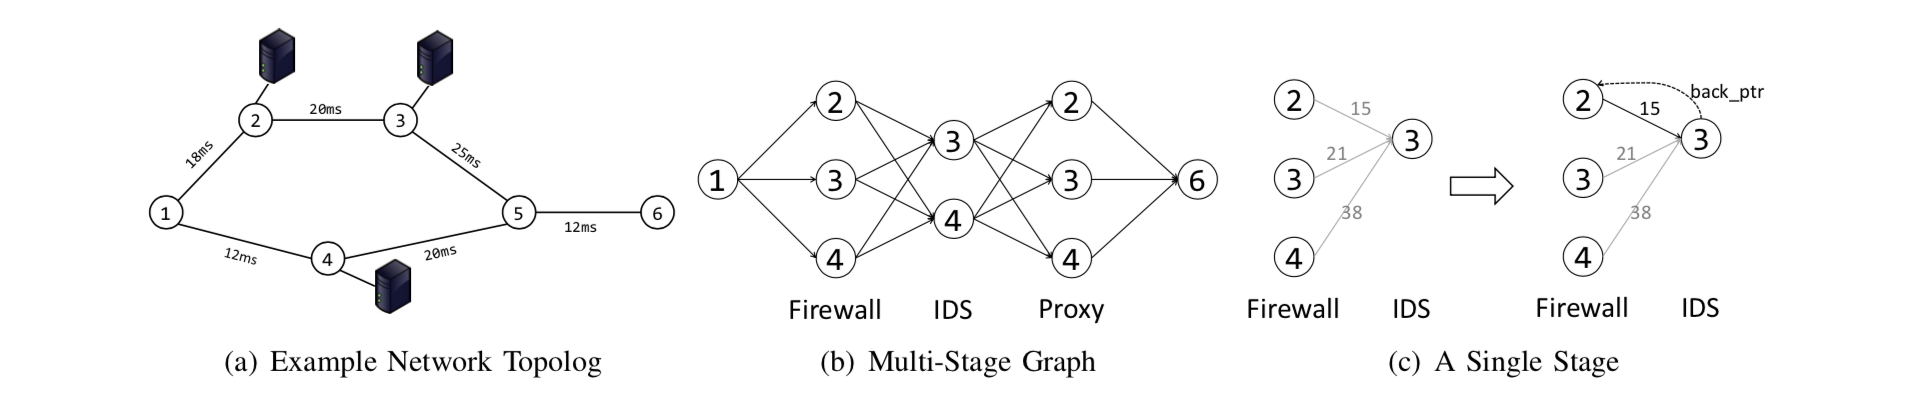
\includegraphics[width=\textwidth]{images/bari.png}
  \caption{Stage transitions of the \cite{Bari2015} algorithm used to build the
  multi-stage placement graph.}
\end{figure}

As a baseline for comparison, we also consider a management-blind variant that
runs the \cite{Bari2015} algorithm with an extra stage appended for the VNFM,
i.e. it places the manager only after the VNF layout is fixed. We use this
disjoint variant in Section~\ref{sec:results} to isolate the benefit of the
management-aware placement in Algorithm~\ref{alg:masman}.

\subsection{Complexity}
For a chain of \(L\) VNFs, the phase-one dynamic program fills an
\(L \times |V^p|\) table and evaluates each entry against every candidate
predecessor, so it costs \(O(L\,|V^p|^2)\) per chain and
\(O(|R|\,L_{\max}\,|V^p|^2)\) over all requests, where \(L_{\max}\) is the longest
chain. The feasibility test at each transition is dominated by a shortest-path
check on the management/service links, bounded by \(O(|E^p|)\). Phase two assigns
an initial manager in \(O(|R|\,|V^p|)\) and then runs \(maxIterations\)
consolidation steps, each \(O(|R|)\). The overall running time is therefore
polynomial in the size of the infrastructure and the request set, in contrast to
the exponential worst case of the exact ILP.


\section{Evaluation and Numerical Results}\label{sec:results}
\subsection{Heuristic vs. the Exact Solver}\label{sec:heuristic-vs-optimal}

We implemented the ILP of Section~\ref{sec:formulation} in IBM CPLEX and use it
both as the optimal baseline and to expose why a heuristic is needed. Two
properties matter: the exact solver does not scale, and MASMAN stays close to its
optimum where it does.

\textbf{Scalability.} Table~\ref{tbl:exact-runtime-topology} reports the optimal
solve time as the fat-tree degree grows, for a fixed load of 8 chains: it rises
from 4~s at \(k = 6\) to 5~min~20~s at \(k = 12\). Fixing the topology at a
12-ary fat tree and increasing the load instead
(Table~\ref{tbl:exact-runtime-chains}), the solve time grows from 5~min~20~s at 8
chains to 16~min~33~s at 11 chains, and exhausts the 12~GB heap (out-of-memory) at
12 chains. The exact solver is therefore confined to small instances, whereas the
heuristic places hundreds of chains (Section~\ref{sec:joint-vs-disjoint}). These
runtimes were measured on 4~vCPUs with 16~GB of RAM and a 12~GB heap, with no
constraint on the VNFM license fee.

\begin{table}[H]
\caption{Optimal solve time vs. fat-tree degree \(k\) (8 chains).}
\label{tbl:exact-runtime-topology}
\begin{tabularx}{0.6\textwidth}{Xr}
\toprule
\textbf{\(k\)-ary fat tree} & \textbf{Time} \\
\midrule
6 & 4 s \\
8 & 7 s \\
10 & 1 min \\
12 & 5 min 20 s \\
\bottomrule
\end{tabularx}
\end{table}

\begin{table}[H]
\caption{Optimal solve time vs. number of chains (12-ary fat tree, 4~vCPU /
16~GB).}
\label{tbl:exact-runtime-chains}
\begin{tabularx}{0.6\textwidth}{Xr}
\toprule
\textbf{Chains} & \textbf{Time} \\
\midrule
8 & 5 min 20 s \\
10 & 7 min 6 s \\
11 & 16 min 33 s \\
12 & out of memory \\
\bottomrule
\end{tabularx}
\end{table}

\textbf{Near-optimality.} On instances the exact solver can handle, we report the
heuristic revenue as a proportion of the optimal revenue
(Table~\ref{tbl:near-optimal}), for 100 chains of length 5--7 at two per-instance
revenue ranges. The management-aware VNF placement reaches 81\% of optimal and the
full method (with Tabu VNFM consolidation) reaches 82\%, against 61\% for the
unmodified Bari~\cite{Bari2015} baseline. The advantage widens as the per-instance
revenue grows, i.e. as accepting each chain becomes more valuable relative to the
VNFM license cost.

\begin{table}[H]
\caption{Heuristic revenue as a percentage of the optimal revenue (100 chains,
length 5--7).}
\label{tbl:near-optimal}
\begin{tabularx}{\textwidth}{Xrrr}
\toprule
\textbf{Revenue per instance} & \textbf{Bari~\cite{Bari2015}} & \textbf{MASMAN (VNF phase)} & \textbf{MASMAN (full)} \\
\midrule
10--20 & 60\% & 65\% & 68\% \\
15--25 & 61\% & 81\% & 82\% \\
\bottomrule
\end{tabularx}
\end{table}

\subsection{Joint vs. Disjoint}\label{sec:joint-vs-disjoint}

We compare the \emph{joint} solution (placing VNFs and their VNFM together)
against the \emph{disjoint} baseline (placing VNFs first and the VNFM afterward),
both solved to optimality with CPLEX. The key effect is one of \emph{feasibility}:
a management-blind disjoint placement can strand whole chains because no
admissible VNFM exists for the chosen VNF layout, so the joint solution accepts
more chains. Crucially, this benefit is \emph{conditional}---it appears only when
the management constraints actually bind, as the two topologies below make clear.
We therefore report chain \emph{acceptance rate} as the primary metric; the
corresponding mean revenue, which only smooths over the mechanism, is tabulated
for reference in Appendix~\ref{sec:revenue-appendix}. We vary the number of
chains; chains are generated randomly with the configuration in
Table~\ref{tbl:chain-config}.

\begin{table}[H]
\caption{Chain configuration.}
\label{tbl:chain-config}
\begin{tabularx}{0.6\textwidth}{lX}
\toprule
\textbf{Property} & \textbf{Value} \\
\midrule
Length & \([4, 7)\) \\
Per-instance cost & \$100 \\
Bandwidth & 250 bps \\
\bottomrule
\end{tabularx}
\end{table}

We evaluate two topologies: a FatTree with \(k = 6\), and a USNet topology with
3--4 nodes attached to each of its points. Each point is the average of 15 CPLEX
runs under a time limit and a 5\% optimality-gap limit.

\subsection{Acceptance Rate: the Feasibility Effect}\label{sec:acceptance}

We report chain \emph{acceptance rate}---the fraction of requested chains that
are admitted---and test each point with a paired Wilcoxon signed-rank test (joint
vs. disjoint on the \emph{same} chain set, 10--15 runs per point).

Two facts stand out. First, the joint solution accepts \(\approx 100\%\) of
chains in \emph{every} regime---it is essentially feasibility-immune, because it
placed the VNFs with management in mind. Second, the disjoint baseline is
\emph{bimodal}: a run either nearly succeeds or collapses, because the post-hoc
manager step is infeasible for the layout the VNF stage happened to choose. The
per-point coefficient of variation (Disjoint CV, up to \(\sim\)80\%) and the
worst single run (Disjoint min, as low as 0\%) expose a spread that the revenue
averages hide. All revenue differences below are significant at \(p < 0.05\)
(paired Wilcoxon).

\begin{table}[H]
\caption{Chain acceptance rate on FatTree (\(k = 6\), default VNFM)---management
binds.}
\label{tbl:acceptance-fattree}
\begin{tabularx}{\textwidth}{Xrrrr}
\toprule
\textbf{Chains} & \textbf{Joint (\%)} & \textbf{Disjoint (\%)} & \textbf{Disjoint min (\%)} & \textbf{Disjoint CV (\%)} \\
\midrule
10 & 100.0 & 46.0 & 0.0 & 69.6 \\
15 & 100.0 & 18.7 & 0.0 & 62.8 \\
20 & 100.0 & 20.3 & 5.0 & 41.6 \\
25 & 100.0 & 31.2 & 8.0 & 78.9 \\
30 & 100.0 & 60.2 & 6.7 & 55.3 \\
35 & 100.0 & 85.7 & 77.1 & 7.0 \\
40 & 100.0 & 83.2 & 62.5 & 15.4 \\
45 & 100.0 & 87.7 & 44.4 & 19.8 \\
50 & 99.9 & 70.5 & 36.0 & 39.3 \\
55 & 100.0 & 61.5 & 23.6 & 47.6 \\
60 & 99.9 & 56.4 & 28.3 & 46.8 \\
65 & 99.9 & 65.6 & 29.2 & 47.6 \\
70 & 100.0 & 53.2 & 25.7 & 53.9 \\
75 & 99.8 & 53.6 & 32.0 & 51.7 \\
80 & 100.0 & 56.0 & 33.8 & 46.2 \\
85 & 100.0 & 50.6 & 31.8 & 48.5 \\
90 & 100.0 & 59.6 & 27.8 & 46.6 \\
\bottomrule
\end{tabularx}
\end{table}

\begin{table}[H]
\caption{Chain acceptance rate on USNet (4-hop manager radius)---management
binds.}
\label{tbl:acceptance-usnet-radius}
\begin{tabularx}{\textwidth}{Xrrrr}
\toprule
\textbf{Chains} & \textbf{Joint (\%)} & \textbf{Disjoint (\%)} & \textbf{Disjoint min (\%)} & \textbf{Disjoint CV (\%)} \\
\midrule
10 & 100.0 & 34.7 & 0.0 & 80.8 \\
15 & 100.0 & 41.8 & 26.7 & 24.4 \\
20 & 100.0 & 42.3 & 25.0 & 22.8 \\
25 & 100.0 & 45.1 & 24.0 & 45.4 \\
30 & 99.8 & 68.7 & 40.0 & 33.0 \\
35 & 100.0 & 94.1 & 85.7 & 4.5 \\
40 & 99.8 & 85.3 & 72.5 & 9.8 \\
45 & 99.9 & 87.1 & 57.8 & 12.6 \\
50 & 99.9 & 93.6 & 88.0 & 2.7 \\
55 & 99.6 & 89.8 & 58.2 & 10.2 \\
60 & 99.6 & 90.3 & 81.7 & 4.3 \\
65 & 99.3 & 88.2 & 47.7 & 12.7 \\
70 & 99.8 & 92.1 & 87.1 & 3.6 \\
75 & 99.4 & 87.7 & 46.7 & 12.8 \\
80 & 99.4 & 91.4 & 86.2 & 3.1 \\
85 & 99.2 & 90.6 & 60.0 & 9.3 \\
90 & 99.3 & 91.7 & 88.9 & 2.1 \\
\bottomrule
\end{tabularx}
\end{table}

\begin{table}[H]
\caption{Chain acceptance rate on USNet (default VNFM)---management slack.}
\label{tbl:acceptance-usnet-slack}
\begin{tabularx}{\textwidth}{Xrrrr}
\toprule
\textbf{Chains} & \textbf{Joint (\%)} & \textbf{Disjoint (\%)} & \textbf{Disjoint min (\%)} & \textbf{Disjoint CV (\%)} \\
\midrule
50 & 100.0 & 100.0 & 100.0 & 0.0 \\
75 & 100.0 & 100.0 & 100.0 & 0.0 \\
100 & 100.0 & 100.0 & 100.0 & 0.0 \\
125 & 100.0 & 100.0 & 100.0 & 0.0 \\
150 & 99.9 & 100.0 & 100.0 & 0.0 \\
\bottomrule
\end{tabularx}
\end{table}

\begin{figure}[H]
\centering
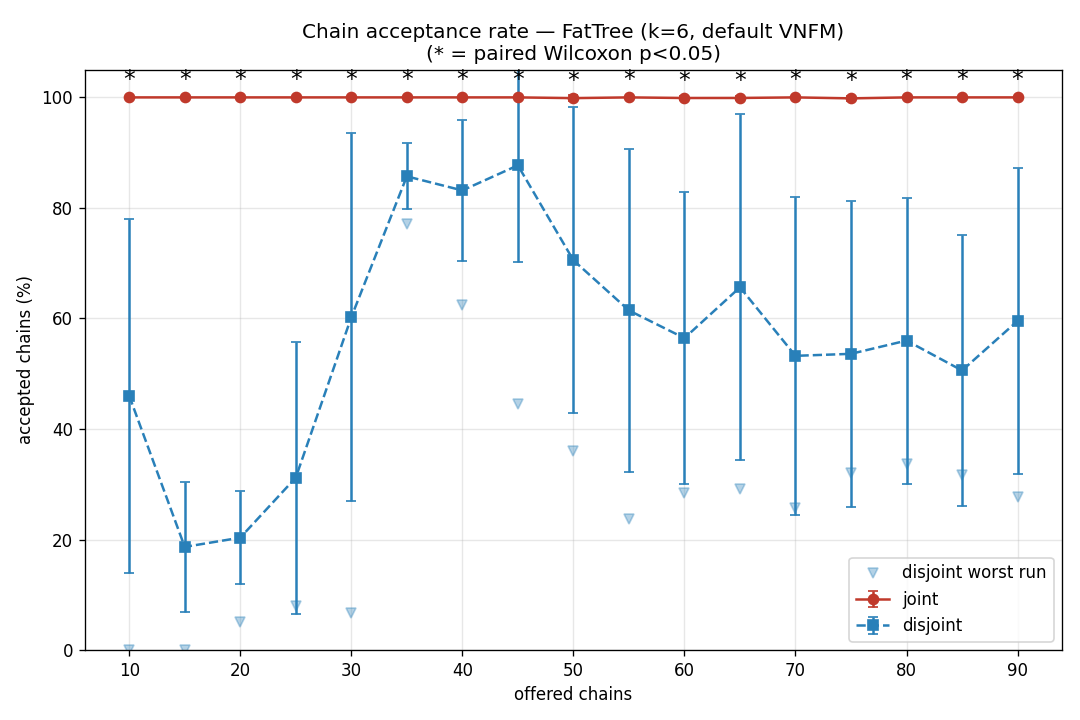
\includegraphics[width=0.32\textwidth]{plots/acceptance-fattree.png}
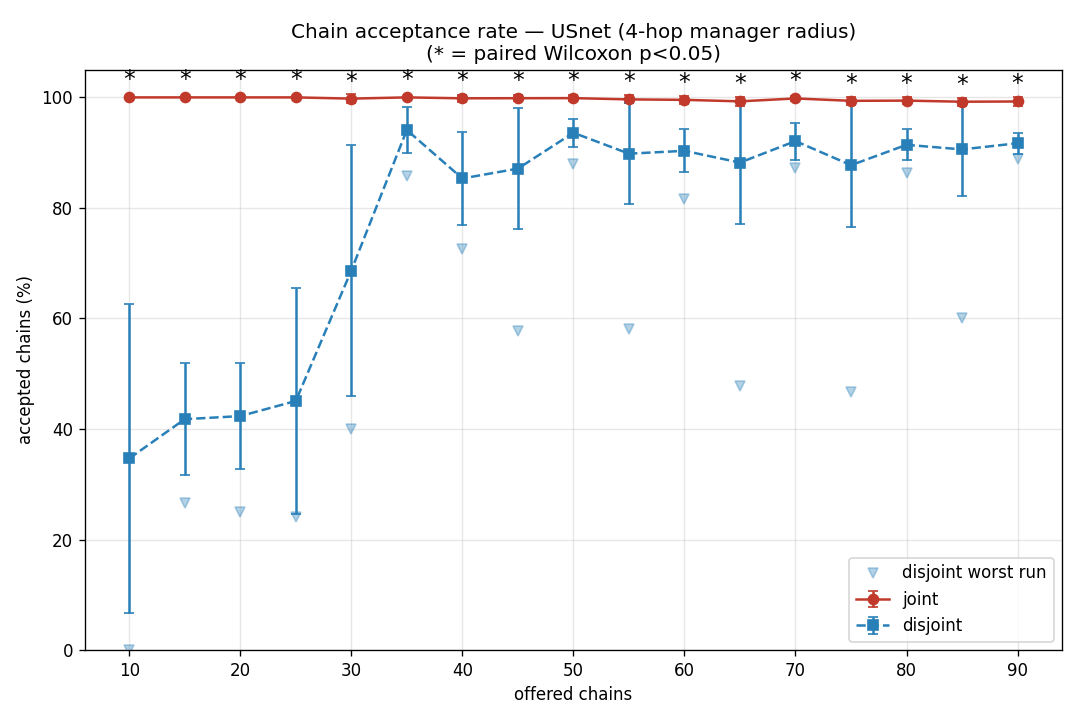
\includegraphics[width=0.32\textwidth]{plots/acceptance-usnet-radius.png}
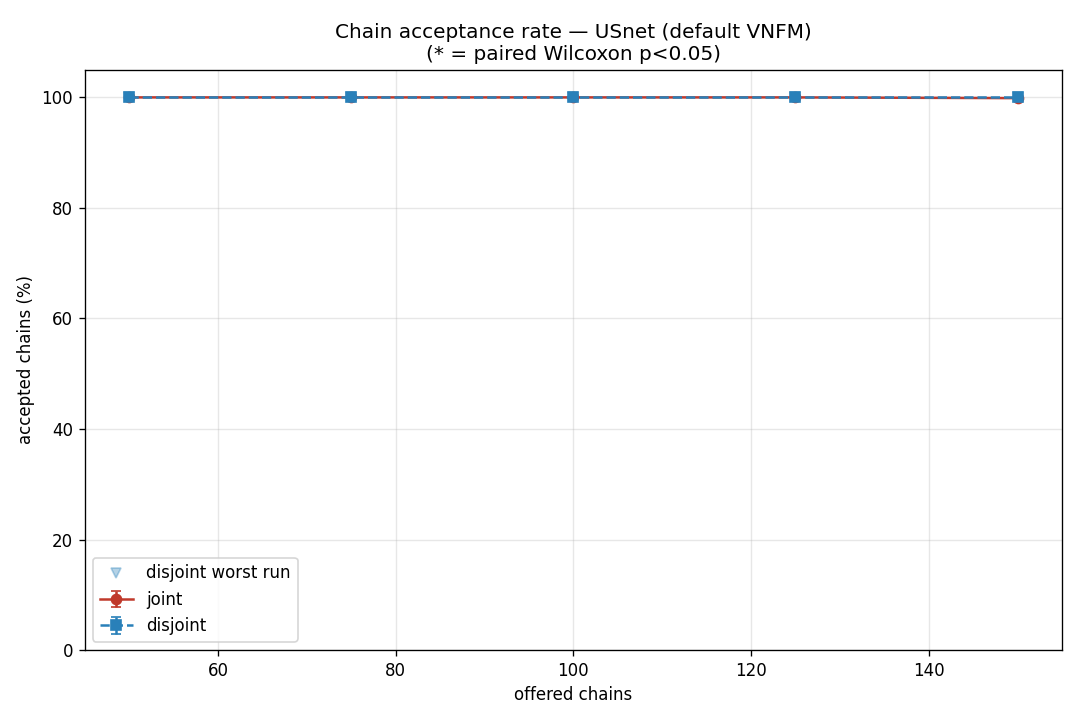
\includegraphics[width=0.32\textwidth]{plots/acceptance-usnet-slack.png}
\caption{Acceptance rate vs. number of chains. Left: FatTree (default VNFM).
Middle: USNet (4-hop radius). Right: USNet (slack management). Joint stays at
\(\approx 100\%\); disjoint collapses precisely where management binds and matches
joint where it does not.}
\label{fig:acceptance}
\end{figure}

On FatTree with the default VNFM, and on USNet once a 4-hop manager radius is
imposed, the management constraint binds and joint placement dominates. In the
slack regime (USNet, default VNFM) disjoint reaches 100\% acceptance with zero
variance, so the joint formulation adds nothing---and, accounting for management
that never binds, it diverts VNF placement enough to be \emph{marginally worse}
on revenue (\(-0.2\%\) to \(-0.9\%\), paired Wilcoxon \(p < 0.01\); see
Appendix~\ref{sec:revenue-appendix}). We keep this null result in deliberately:
it delimits the regime in which joint placement is worth the extra coupling. Note
that the same USNet topology moves from ``no difference'' to a clear joint
advantage by tightening a single management parameter---the manager radius---which
is the central message of this comparison.

\subsection{When Joint Placement Matters: a Controlled Sweep}\label{sec:sweep}

The comparisons above show \emph{that} the advantage is conditional; a controlled
sweep on the 15-node example topology isolates \emph{why}. Here the joint method
is the management-aware heuristic (Bari) and the disjoint method is the same
pipeline with management-blind VNF placement, with 8 paired runs per point.

\textbf{The management constraint is the cause.} Holding the network and chains
fixed, we toggle the per-node co-location (notManagerNodes) management constraint
on and off (Table~\ref{tbl:sweep-constraint}, Figure~\ref{fig:sweep-constraint}).
With it \emph{on}, the joint method leads disjoint by 12--19 percentage points of
acceptance at low load; with it \emph{off}, disjoint matches joint exactly (gap 0)
at every load. Joint acceptance is identical in both columns---it is immune by
construction. The gap also decays to 0 as load rises and raw VNF resources, not
management, become the bottleneck.

\begin{table}[H]
\caption{Toggling the management constraint (controlled A/B). The joint advantage
exists if and only if the constraint binds, and decays under load.}
\label{tbl:sweep-constraint}
\begin{tabularx}{\textwidth}{Xrrrrr}
\toprule
\textbf{Load} & \textbf{Joint (\%)} & \textbf{Disjoint on (\%)} & \textbf{Gap on} & \textbf{Disjoint off (\%)} & \textbf{Gap off} \\
\midrule
2 & 100.0 & 87.5 & 12.5 & 100.0 & 0.0 \\
3 & 100.0 & 83.3 & 16.7 & 100.0 & 0.0 \\
4 & 100.0 & 81.2 & 18.8 & 100.0 & 0.0 \\
5 & 100.0 & 82.5 & 17.5 & 100.0 & 0.0 \\
6 & 93.8 & 77.1 & 16.7 & 93.8 & 0.0 \\
7 & 87.5 & 75.0 & 12.5 & 87.5 & 0.0 \\
8 & 78.1 & 73.4 & 4.7 & 78.1 & 0.0 \\
9 & 70.8 & 69.4 & 1.4 & 70.8 & 0.0 \\
10 & 63.8 & 62.5 & 1.2 & 63.8 & 0.0 \\
12 & 54.2 & 54.2 & 0.0 & 54.2 & 0.0 \\
\bottomrule
\end{tabularx}
\end{table}

\begin{figure}[H]
\centering
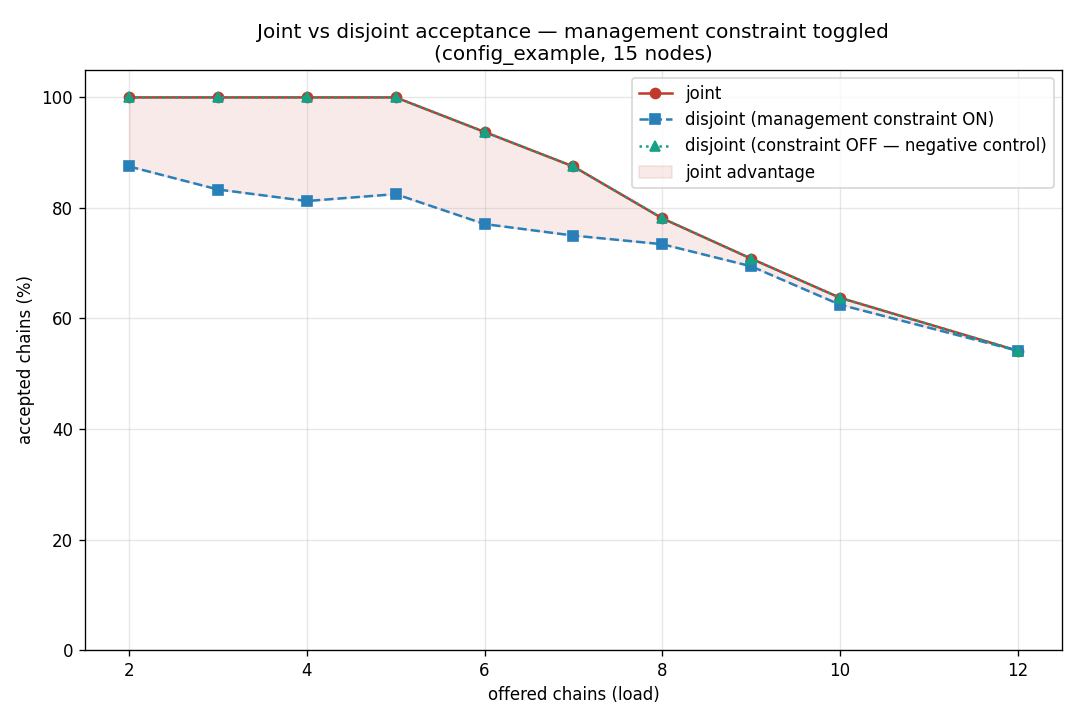
\includegraphics[width=0.7\textwidth]{plots/sweep-constraint.png}
\caption{Acceptance vs. load with the management constraint on vs. off. The
joint--disjoint gap appears only when the constraint is present.}
\label{fig:sweep-constraint}
\end{figure}

\textbf{Manager capacity is not the lever (negative control).} Sweeping manager
capacity over two orders of magnitude barely moves the gap
(Table~\ref{tbl:sweep-capacity}): on this topology capacity does not bind, so it
is not what drives the joint advantage. The binding lever here is the co-location
constraint; on the full topologies it is the manager radius
(Section~\ref{sec:acceptance}).

\begin{table}[H]
\caption{Manager capacity as a non-binding lever (negative control). The gap is
essentially constant from capacity 1 to 100.}
\label{tbl:sweep-capacity}
\begin{tabularx}{0.7\textwidth}{Xrrr}
\toprule
\textbf{Capacity} & \textbf{Joint (\%)} & \textbf{Disjoint (\%)} & \textbf{Gap (pp)} \\
\midrule
1 & 93.8 & 77.1 & 16.7 \\
2 & 93.8 & 81.2 & 12.5 \\
3 & 93.8 & 77.1 & 16.7 \\
5 & 93.8 & 81.2 & 12.5 \\
10 & 93.8 & 77.1 & 16.7 \\
20 & 93.8 & 77.1 & 16.7 \\
100 & 93.8 & 79.2 & 14.6 \\
\bottomrule
\end{tabularx}
\end{table}

Together these results turn a soft comparison into a characterization: joint
placement does not make good layouts better; it makes infeasible layouts
feasible---exactly when a management constraint binds, and not otherwise.


\section{Conclusions}\label{sec:conclusion}
We considered, for the first time, the joint deployment of service function
chains and the placement of their VNF Managers (JSD-MP). We formulated the
problem as an ILP, showed its NP-hardness, and proposed MASMAN, a
polynomial-time heuristic that is management-aware during VNF placement and
consolidates managers with Tabu search. Our evaluation shows the heuristic stays
within roughly 18\% of the optimal revenue while scaling well beyond the reach of
the exact solver, and that the value of joint placement is a feasibility effect
that is large exactly when management constraints bind. Future work includes an
online variant in which requests arrive over time, reliability-aware manager
placement with backup managers, and tighter approximation guarantees for the
manager-placement subproblem (which is a capacitated facility-location problem
with a coverage radius).

\vspace{6pt}

\authorcontributions{Conceptualization, P.A. and B.B.; methodology, P.A. and
B.B.; software, P.A.; validation, P.A. and B.B.; formal analysis, P.A.;
investigation, P.A.; writing---original draft preparation, P.A.;
writing---review and editing, B.B.; supervision, B.B. All authors have read and
agreed to the published version of the manuscript.}

\funding{This research received no external funding.}

\conflictsofinterest{The authors declare no conflict of interest.}

\appendixtitles{yes}
\appendix
\section{Revenue Tables}\label{sec:revenue-appendix}
For reference, we tabulate the mean revenue underlying the acceptance-rate
results of Section~\ref{sec:acceptance}. Revenue tracks acceptance but smooths
over the bimodal collapse of the disjoint baseline, which is why we report
acceptance as the primary metric. Each value is the average of 15 CPLEX runs
under a time and optimality-gap limit.

\begin{table}[H]
\caption{Revenue of joint vs. disjoint on FatTree (\(k = 6\), default VNFM).}
\label{tbl:fattree}
\begin{tabularx}{0.7\textwidth}{Xrr}
\toprule
\textbf{Chains} & \textbf{Joint} & \textbf{Disjoint} \\
\midrule
10 & 4453 & 1913 \\
15 & 6587 & 1000 \\
20 & 8887 & 1593 \\
25 & 11{,}133 & 3267 \\
30 & 13{,}327 & 7907 \\
35 & 15{,}467 & 13{,}073 \\
40 & 17{,}973 & 14{,}687 \\
45 & 20{,}147 & 17{,}553 \\
50 & 22{,}440 & 15{,}633 \\
55 & 24{,}447 & 14{,}613 \\
60 & 26{,}940 & 14{,}713 \\
65 & 29{,}313 & 18{,}887 \\
70 & 31{,}487 & 16{,}313 \\
75 & 33{,}713 & 17{,}340 \\
80 & 36{,}253 & 19{,}553 \\
85 & 37{,}847 & 18{,}540 \\
90 & 40{,}500 & 23{,}360 \\
\bottomrule
\end{tabularx}
\end{table}

\begin{figure}[H]
\centering
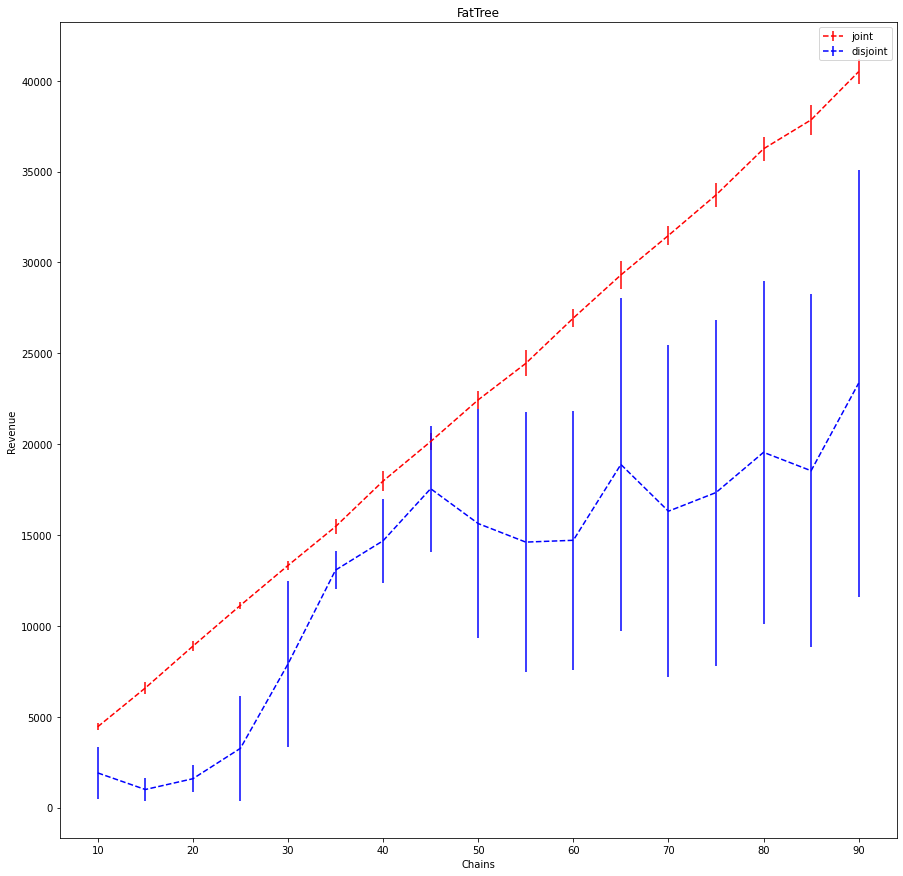
\includegraphics[width=0.7\textwidth]{plots/joint-vs-disjoint-fattree.png}
\caption{Revenue of joint vs. disjoint on FatTree (\(k = 6\)).}
\label{fig:fattree}
\end{figure}

With the \emph{default} (slack) management settings the joint and disjoint
solutions earn essentially identical revenue on USNet
(Table~\ref{tbl:usnet-slack}, Figure~\ref{fig:usnet-slack}): the topology can
manage every chain, so the management constraint does not bind.

\begin{table}[H]
\caption{Revenue of joint vs. disjoint on USNet (slack management).}
\label{tbl:usnet-slack}
\begin{tabularx}{0.7\textwidth}{Xrr}
\toprule
\textbf{Chains} & \textbf{Joint} & \textbf{Disjoint} \\
\midrule
50 & 23{,}000 & 23{,}010 \\
75 & 34{,}180 & 34{,}260 \\
100 & 45{,}430 & 45{,}560 \\
125 & 57{,}180 & 57{,}380 \\
150 & 68{,}750 & 69{,}360 \\
\bottomrule
\end{tabularx}
\end{table}

\begin{figure}[H]
\centering
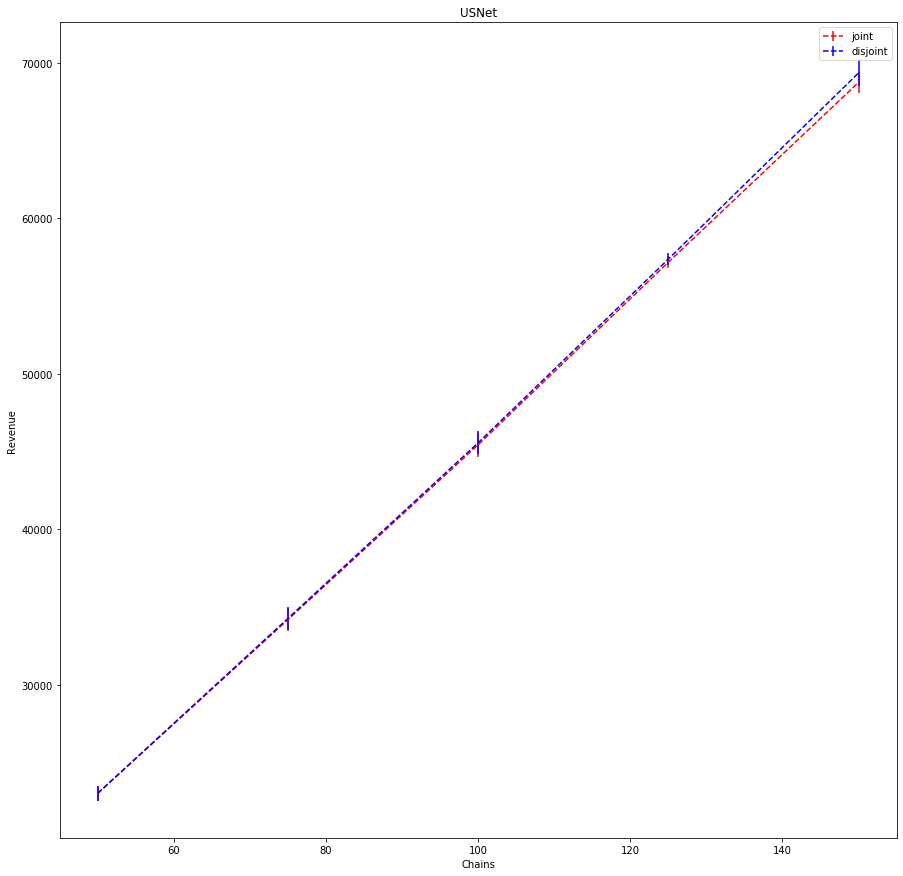
\includegraphics[width=0.7\textwidth]{plots/joint-vs-disjoint-usnet-1.png}
\caption{Revenue of joint vs. disjoint on USNet (slack management).}
\label{fig:usnet-slack}
\end{figure}

When the manager radius is tightened to 4 hops the constraint binds and the joint
advantage reappears in revenue as well (Table~\ref{tbl:usnet-tight},
Figure~\ref{fig:usnet-tight}).

\begin{table}[H]
\caption{Revenue of joint vs. disjoint on USNet (4-hop management radius).}
\label{tbl:usnet-tight}
\begin{tabularx}{0.7\textwidth}{Xrr}
\toprule
\textbf{Chains} & \textbf{Joint} & \textbf{Disjoint} \\
\midrule
10 & 4473 & 1420 \\
15 & 6927 & 2733 \\
20 & 8940 & 3533 \\
25 & 11{,}133 & 4833 \\
30 & 13{,}313 & 9020 \\
35 & 15{,}487 & 14{,}693 \\
40 & 17{,}913 & 15{,}433 \\
45 & 19{,}813 & 17{,}587 \\
50 & 22{,}213 & 21{,}020 \\
55 & 24{,}113 & 21{,}867 \\
60 & 26{,}640 & 24{,}547 \\
65 & 28{,}833 & 25{,}760 \\
70 & 31{,}360 & 29{,}420 \\
75 & 33{,}140 & 29{,}660 \\
80 & 35{,}687 & 33{,}320 \\
85 & 37{,}600 & 34{,}987 \\
90 & 39{,}840 & 37{,}473 \\
\bottomrule
\end{tabularx}
\end{table}

\begin{figure}[H]
\centering
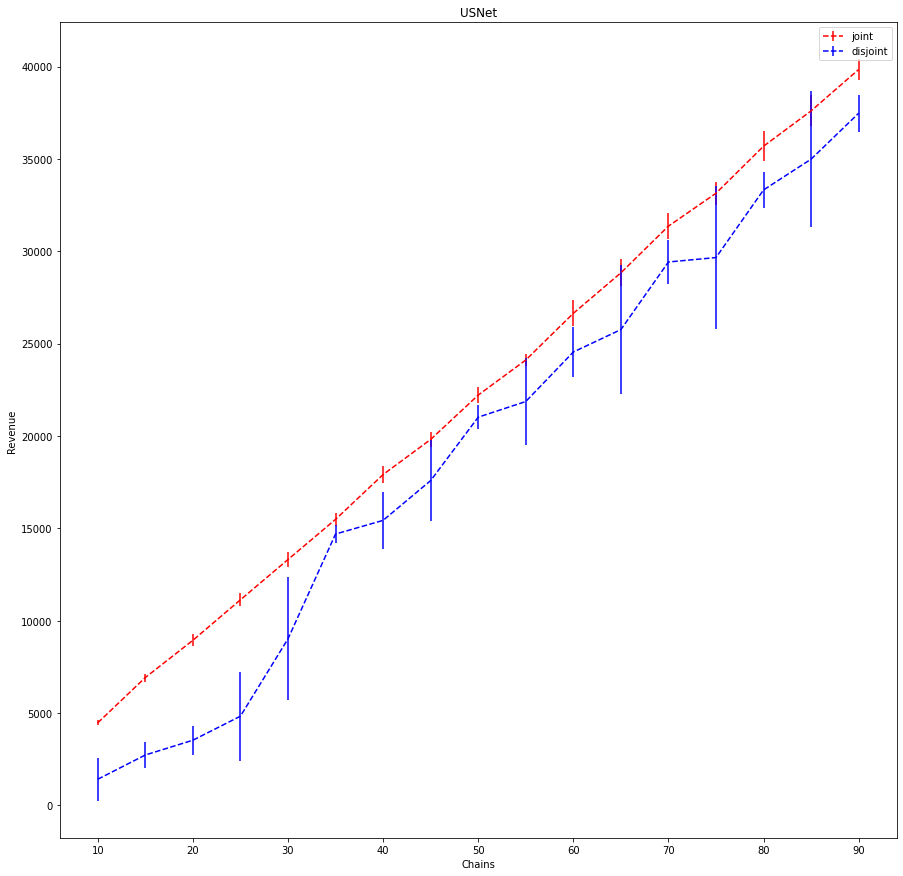
\includegraphics[width=0.7\textwidth]{plots/joint-vs-disjoint-usnet-2.png}
\caption{Revenue of joint vs. disjoint on USNet (4-hop management radius).}
\label{fig:usnet-tight}
\end{figure}


\reftitle{References}
\externalbibliography{yes}
\bibliography{references}

\end{document}
